
\section{Methods}
\label{sec5:methods}

This section describes the hardware, simulation and control of our robot,
the damage scenarios it faces and its options for recovery: 
shapeshifting and controller adaptation.
We also define a tripartite classification|of `structure', `shape' and `configuration'|that forms the basis of our argument, which is, briefly, that the way in which our robot recovers from damage|shape change|was outside the scope of any robot previously reported in the literature.


\subsection*{The source code.}
\href{https://github.com/skriegman/2019-RSS}{\textcolor{blue}{\textbf{\texttt{github.com/skriegman/2019-RSS}}}}



\subsection*{The robot.}
\label{sec5:robot}


% Blue VoxelBot
\begin{wrapfigure}{r}{0.4\linewidth}
\vspace{-14pt}
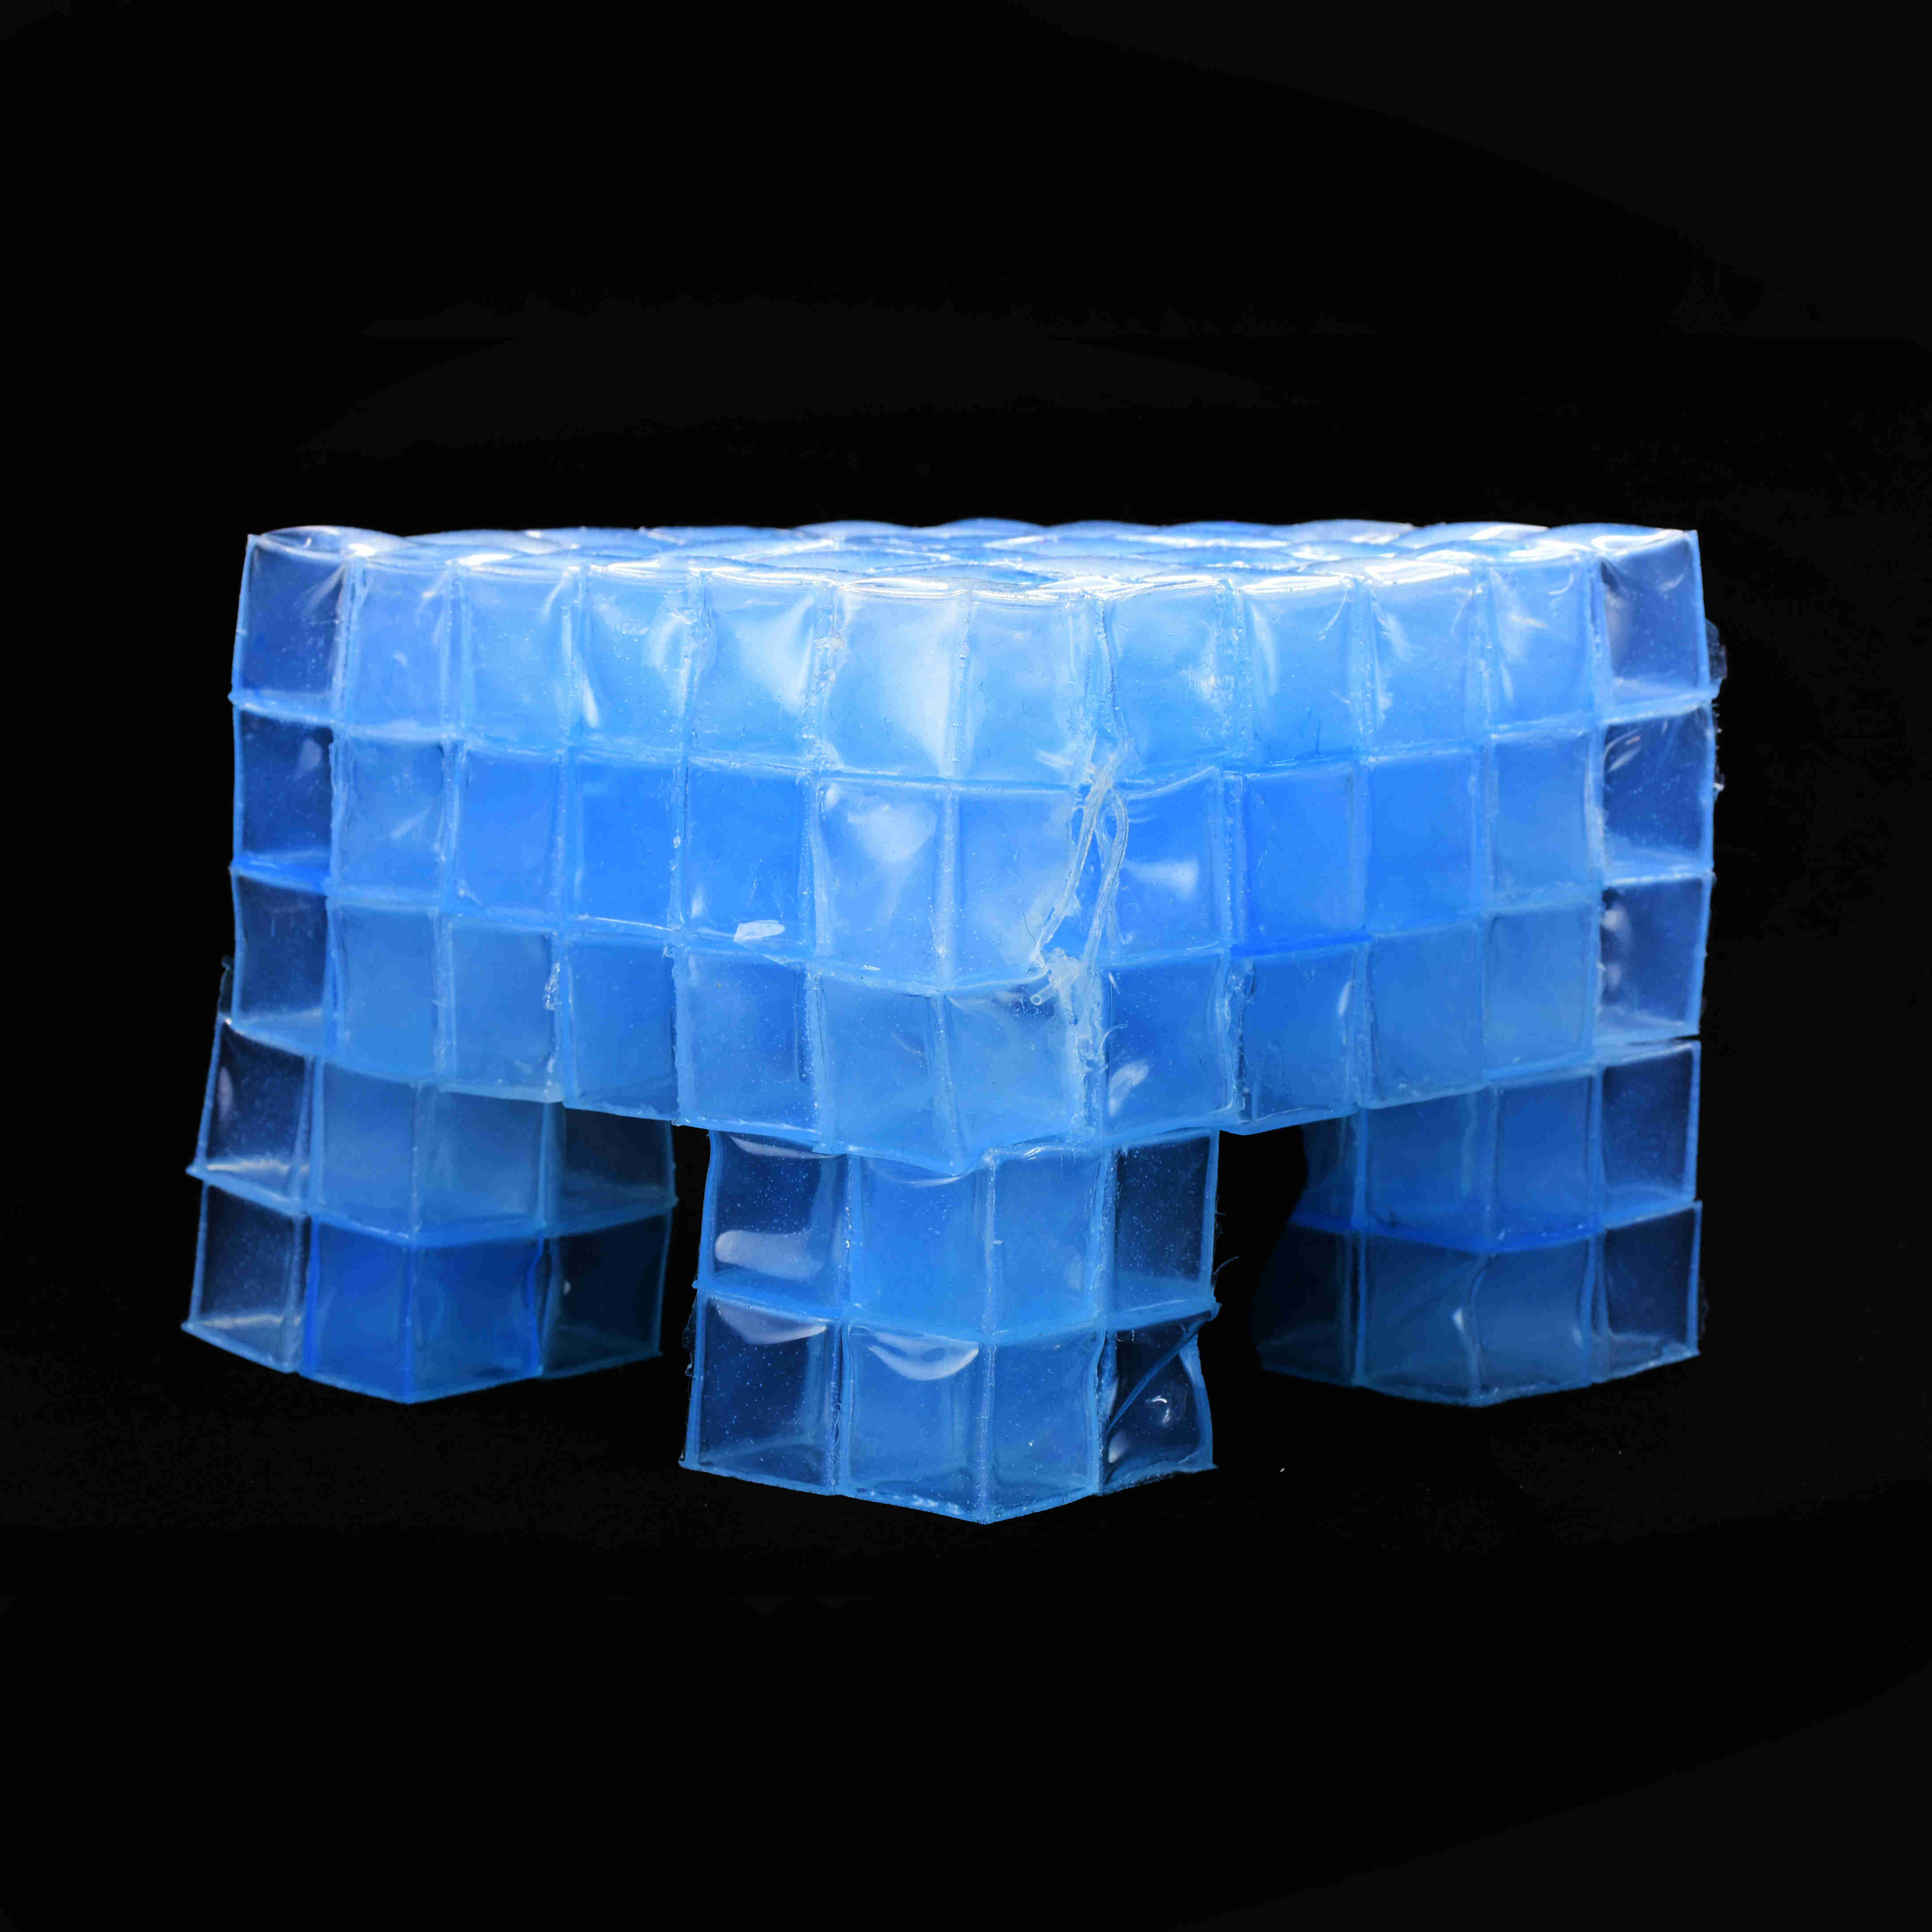
\includegraphics[trim={0 16em 0 17em},clip,width=\linewidth]{Chapter05/fig/DSC_8734_crop-min.jpg}
\vspace{-18pt}
\caption{The blue robot, made from thin-walled inflatable elastomer voxels.}
\label{fig5:blue_quad}
\vspace{-1em}
\end{wrapfigure}



The robot is an isobilaterally symmetrical quadruped constructed from 140 inflatable silicone ``voxels'' 
(Figs.~\ref{fig5:teaser}f and~\ref{fig5:blue_quad}).
We here present a method for creating air-filled voxel membranes with relatively uniform thickness.


Creating thin, hollow 3D silicone structures is challenging due to several factors, including mold precision and potential for damage during release from molds. One effective but labor-intensive method is to make the 3D shapes by adhering 2D films at their joints \cite{morin_elastomeric_2014}. Here, inspired by a scalable 2-axis rotational molding technique \cite{zhao_scalable_2015}, we employ a \mbox{1-axis} rotational drip-molding machine.

First, silicone (Dragon Skin 10 Fast; Smooth-On, Inc.) was poured into an open-face acrylic mold and a tongue depressor was used to roughly spread the silicone along the walls. The mold was then attached to the rotational molding machine with the rotation axis oriented downward at 45 degrees relative to horizontal, and run through cycles comprising a 90\textdegree~turn, stopping for 45 seconds after each turn to allow the silicone to flow and evenly coat each side. Excess silicone dripped out of the mold, leaving a thickness which was dependent on several interrelated factors including the cure time, viscosity, and the interaction between the silicone and acrylic.

After the silicone cured, excess material was cut away. A silicone base-layer was then rod-coated onto a flat acrylic sheet. Next, the bottomless cubes were placed on the base-layer and allowed to cure, sealing air inside each voxel. The voxels were then cut from the sheet and a small hole was punched in each voxel for tubing. Finally, silicone tubes were inserted and bonded with Sil-Poxy (Smooth-On, Inc.).

The overall robot consists of a $6\times6\times3$ voxel torso and four removable $2\times2\times2$ voxel legs (Figs.~\ref{fig5:teaser}f-j  and~\ref{fig5:blue_quad}). 
Sil-Poxy and Ecoflex 00-50 were used to improve adhesion between voxels. 
To explore the effect of layer thickness on the range of attainable morphologies,
two versions of the robot were fabricated:
The {\color{blue}\textbf{blue robot}} (Fig.~\ref{fig5:blue_quad}) consists of voxels made with one layer of silicone, while the {\color{purple}\textbf{purple robot}} \mbox{(Fig.~\ref{fig5:teaser}f-j)} consists of thicker-walled voxels made with two layers of silicone. 

Individual cubic voxels were manually inflated at pressures less than 20~kPa, and approached a spherical shape as pressure increased. 
When patterned together into a robot, selective inflation of a subset of voxels induces overall robot shape change. 
To reduce friction and weight effects in the robots, they were placed on top of a glass crystallizing dish, which lifted their legs off the table surface.
While this arrangement made motion difficult, it allowed us to conduct a preliminary investigation of the feasibility of transferring simulated shape change to a physical system. 
In future implementations, the manual inflation could be replaced by pressure regulators~\cite{booth_addressable_2018}, allowing the robot to approach the continuous control achievable in simulation.

To understand some of the trade-offs between design parameters, consider a spherical pressure vessel in uniform free expansion:
\begin{equation}
    \label{eq5:pressure vessel}
    p=\frac{2 E \cdot \epsilon \cdot t}{r} = \frac{2 E \cdot \epsilon \cdot t_0 \cdot (1-\delta)}{r_0-\epsilon},
\end{equation}
where $t_0$ [m] is the thickness of the pressure vessel, $r_0$~[m] is the radius, $\epsilon$ is the linear strain due to expansion, $E$ [MPa] is Young's modulus, and $\delta$ is the radial strain (which is determined from $\epsilon$ and the material's Poisson's ratio).
Note that each voxel can push outward with a force proportional to the pressure. Examining Eq.~\ref{eq5:pressure vessel}, we see that at a given strain rate and initial dimensions, the internal pressure scales linearly with both thickness and modulus. Thus, when choosing thickness of voxels, there was a tradeoff between weight and internal pressure: doubling the wall thickness doubled weight, in exchange for doubled operational pressure.



\subsection*{The simulation.}


% \definecolor{darkgray}{HTML}{606060}
% \definecolor{darkblue}{HTML}{003366}
% \definecolor{darkred}{HTML}{990000}
\begin{wrapfigure}{r}{0.4\linewidth}
\vspace{-1em}
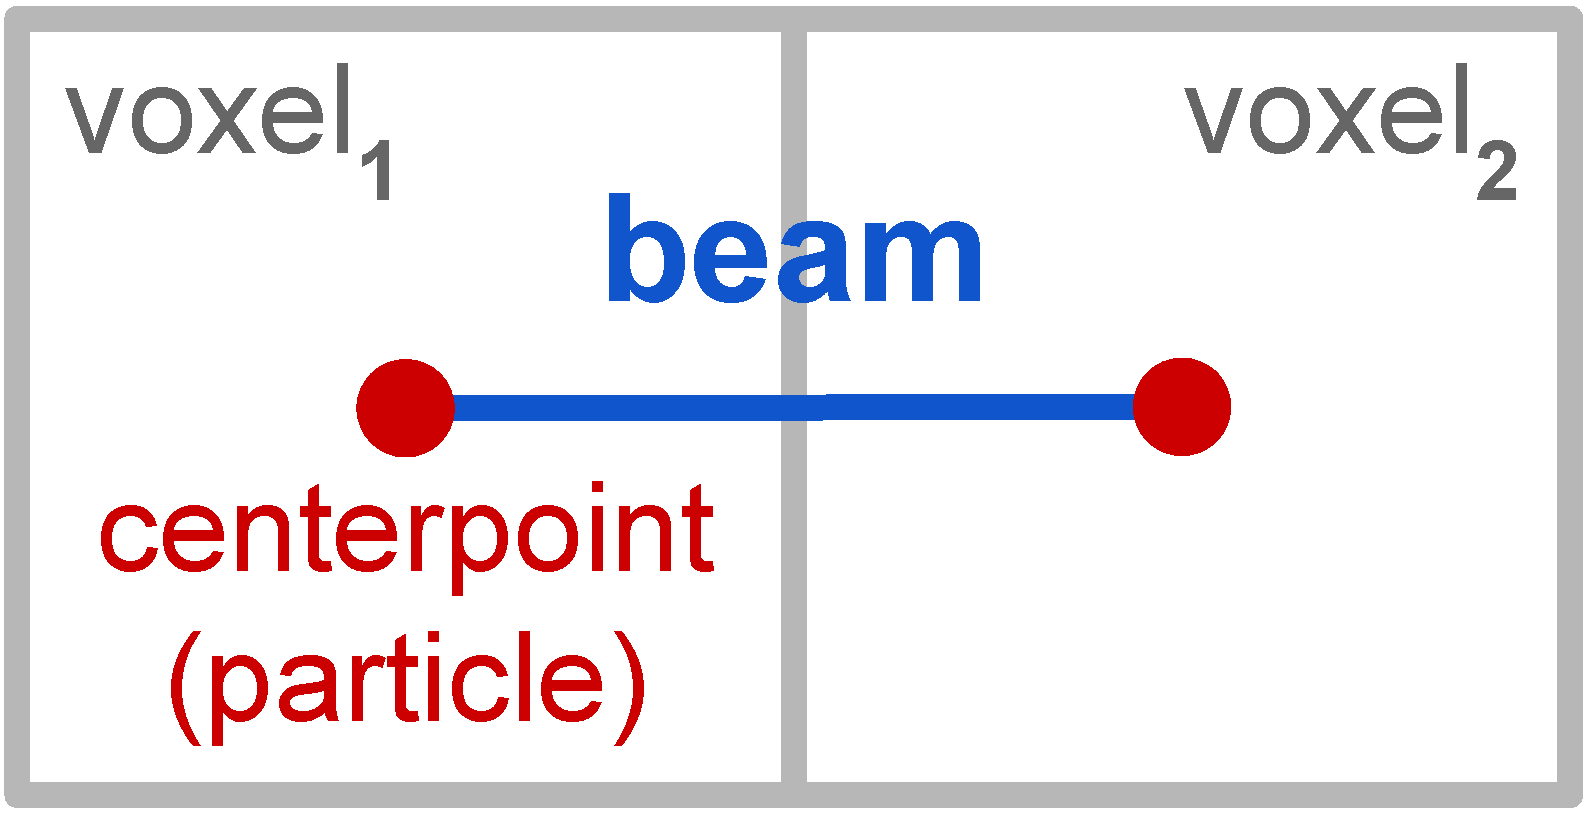
\includegraphics[trim={0 0 0 0},clip,width=\linewidth]{Chapter05/fig/two_cubes.pdf}\\
\vspace{-19pt}
\caption{Voxels are simulated by beams (springs) and particles (masses).
}
\label{fig:voxcad}
\vspace{-1em}
\end{wrapfigure}

To simulate the robot, we use the voxel-based physics engine \textit{Voxelyze} \cite{hiller2014dynamic},
which simulates elastic voxels using two elements: particles and beams.
Particles have mass and rotational inertia, and are connected on a cartesian grid by spring-like beams (with translational and rotational stiffness).
For visualization and reference, part of a voxel mesh is drawn around this structure such that each voxel has a single particle at its center (Fig.~\ref{fig5:voxcad}).

Two adjacent voxels are connected, centerpoint to centerpoint (i.e.,~particle to particle), by a single, shared beam.
Material properties (e.g.,~volume and elasticity) are specified at the particles but implemented as attributes of beams (e.g.,~their rest length, and how easily they twist and stretch).
Where two adjacent particles disagree in their ``desired'' attributes of a shared beam, an average is taken.

A beam exits a voxel normal to, and in the center of, one of the voxel's faces.
Although the mesh is drawn such that voxel edges bend around the underlying beam-mass network (see,~e.g.,~Fig.~\ref{fig5:teaser}), a spherical envelope is used for collision detection, thus approximating the spherical expansion of the physical voxels (with maximal expansion occurring at the center of each face).
For more details see \cite{hiller2014dynamic}.


\subsection*{The structure and shape of a robot.}

The \textbf{structure}, $\mathbb{S}$,
of a robot is determined by the number and placement of voxels, and simulated by the presence and absence of particles on a regular grid in the workspace.
Let the bit value $v_i$ denote the presence ($v_i=1$) or absence ($v_i=0$) of a voxel at index~$i$.
The structure,
\begin{equation}
    \label{eq5:structure}
    \mathbb{S} = \{i : v_i = 1 \} ,
\end{equation}
is thus a set of voxel coordinates.

The \textbf{shape}, $\mathcal{S}$,
of a robot is determined by the resting volume of each voxel, which is expressed in simulation as the resting (or, equilibrium) lengths of the beams connecting adjacent particles, and in reality as a resting pressure within each voxel (though the exact pressure, $p_i$, is not measured here).
Let the floating point value $b_i$ denote the beam rest length stored at the $i$-th simulated voxel.
The shape,
\begin{equation}
    \label{eq5:shape}
    \mathcal{S}_{\text{sim}} = \{b_i : i \in \mathbb{S} \} \; \sim \; \mathcal{S}_{\text{real}} = \{p_i : i \in \mathbb{S} \} ,
\end{equation}
is thus a set of voxel resting volumes.

The robot has a quadrupedal predamage structure (Figs.~\ref{fig5:teaser}a,f and~\ref{fig5:blue_quad}) with atmospheric voxel resting pressure, which is approximated by nominal beam rest lengths of 1~cm.
Damage removes structure (voxels) (Fig.~\ref{fig5:teaser}b).
Postdamage structural deformation|shape change|is executed by pressure changes in the remnant structure (i.e.,~mutations in $\mathcal{S}_{\text{real}}$) \mbox{(Fig.~\ref{fig5:teaser}h-j)} and approximated by local adjustments in the remaining beam-mass network (i.e.,~mutations in $\mathcal{S}_{\text{sim}}$) (Fig.~\ref{fig5:teaser}c-e).
The mechanical structure and its resting shape are fixed prior to behavior during the evaluation period (20 actuation cycles).


\subsection*{The controller and configuration of a robot.}
\label{sec5:methods:controller}


The controllers continuously reconfigure the volume of a given mechanical structure during the evaluation period.
We here consider open loop control of 
$\pm0.5$ cm$^3$ volumetric change ($\pm50\%$ from nominal),
at each voxel, with a phase offset relative to a central pattern generator, for 4~sec.

Controllers are here encoded as neural networks that map the indices of voxels in 3D space (Eq.~\ref{eq5:structure}) to a phase offset value, $\phi_i$, between $-2\pi$ and $2\pi$.
We chose this particular encoding, which is commonly referred to as a Compositional Pattern-Producing Network, or CPPN \cite{stanley2007compositional},
because spatial regularities (in structure and actuation) are known to facilitate locomotion.
(For more details about this encoding, see \cite{cheney2013unshackling}.)


The instantaneous \textbf{configuration}, 
$\mathcal{C}$,
of a robot is determined by an oscillating adjustment to the volume (and thus pressure) of each voxel,
centered around its shape $\mathcal{S}$.
In simulation, rest lengths are
periodically varying \mbox{($f=$ 5~Hz)} around their baseline, $b_i\,$,
with constant amplitude
\mbox{($A\approx$~0.145~cm)}, but damped by $\xi$.
% (Note how $[1+A]^3-1=50\%$ volumetric change.)
Damping prevents contracting voxels from overlapping by decreasing their oscillation amplitude as their rest length approaches a lower bound of $b_i=0.25$~cm.

The instantaneous adjustment to the rest length of the $i$-th simulated voxel, at time~$t$, is thus:
\begin{equation}
\label{eq5:beam_actuation}
\psi_i(t) = A \cdot \sin(2\pi f t + \phi_i) \cdot \xi(b_i) ,
\end{equation}
where:
\begin{equation}
\label{eq5:beam_damp}
\xi(b) = \min\left[ 1,\; \frac{4b - 1}{3} \right] .
\end{equation}
The configuration,
\begin{equation}
\label{eq5:beam_configuration}
\mathcal{C}_{\text{sim}}(t) = \{b_i + \psi_i(t) : i \in \mathbb{S} \} ,
% \sim \mathcal{C}_{\text{real}}(t) = \{p_i + \psi_i'(t) : i \in \mathbb{S} \}
\end{equation}
is thus a cyclical adjustment in the rest length between adjacent simulated voxels (implemented when computing the elastic force between them) throughout a structure $\mathbb{S}$ with shape $\mathcal{S}_{\text{sim}}$.


Although simple, open loop control has the ability to produce complex behaviors,
such as symmetrical and asymmetrical gaits (from patches of voxels that oscillate in counter-phase), or propagating waves of excitation (from a sequence of voxels with increasing or decreasing phase offsets).
Indeed, it is well known that central pattern generators in the mammalian spinal cord (and elsewhere in invertebrate systems) produce the basic, rhythmic motor patterns of locomotion, such as stepping, independently of sensory input \cite{goulding2009circuits}.


\subsection*{The damage scenarios.}


We here consider nine damage scenarios|we amputate: (i) half of a leg; (ii) one entire leg, (iii) two adjacent legs, (iv) two diagonal legs, (v) three legs, (vi) all four legs; (vii) one quarter of the robot's body, (viii) one half of the body, and (ix) three quarters of the body.

\begin{figure}[h]
\begin{center}
% \vspace{-6pt}
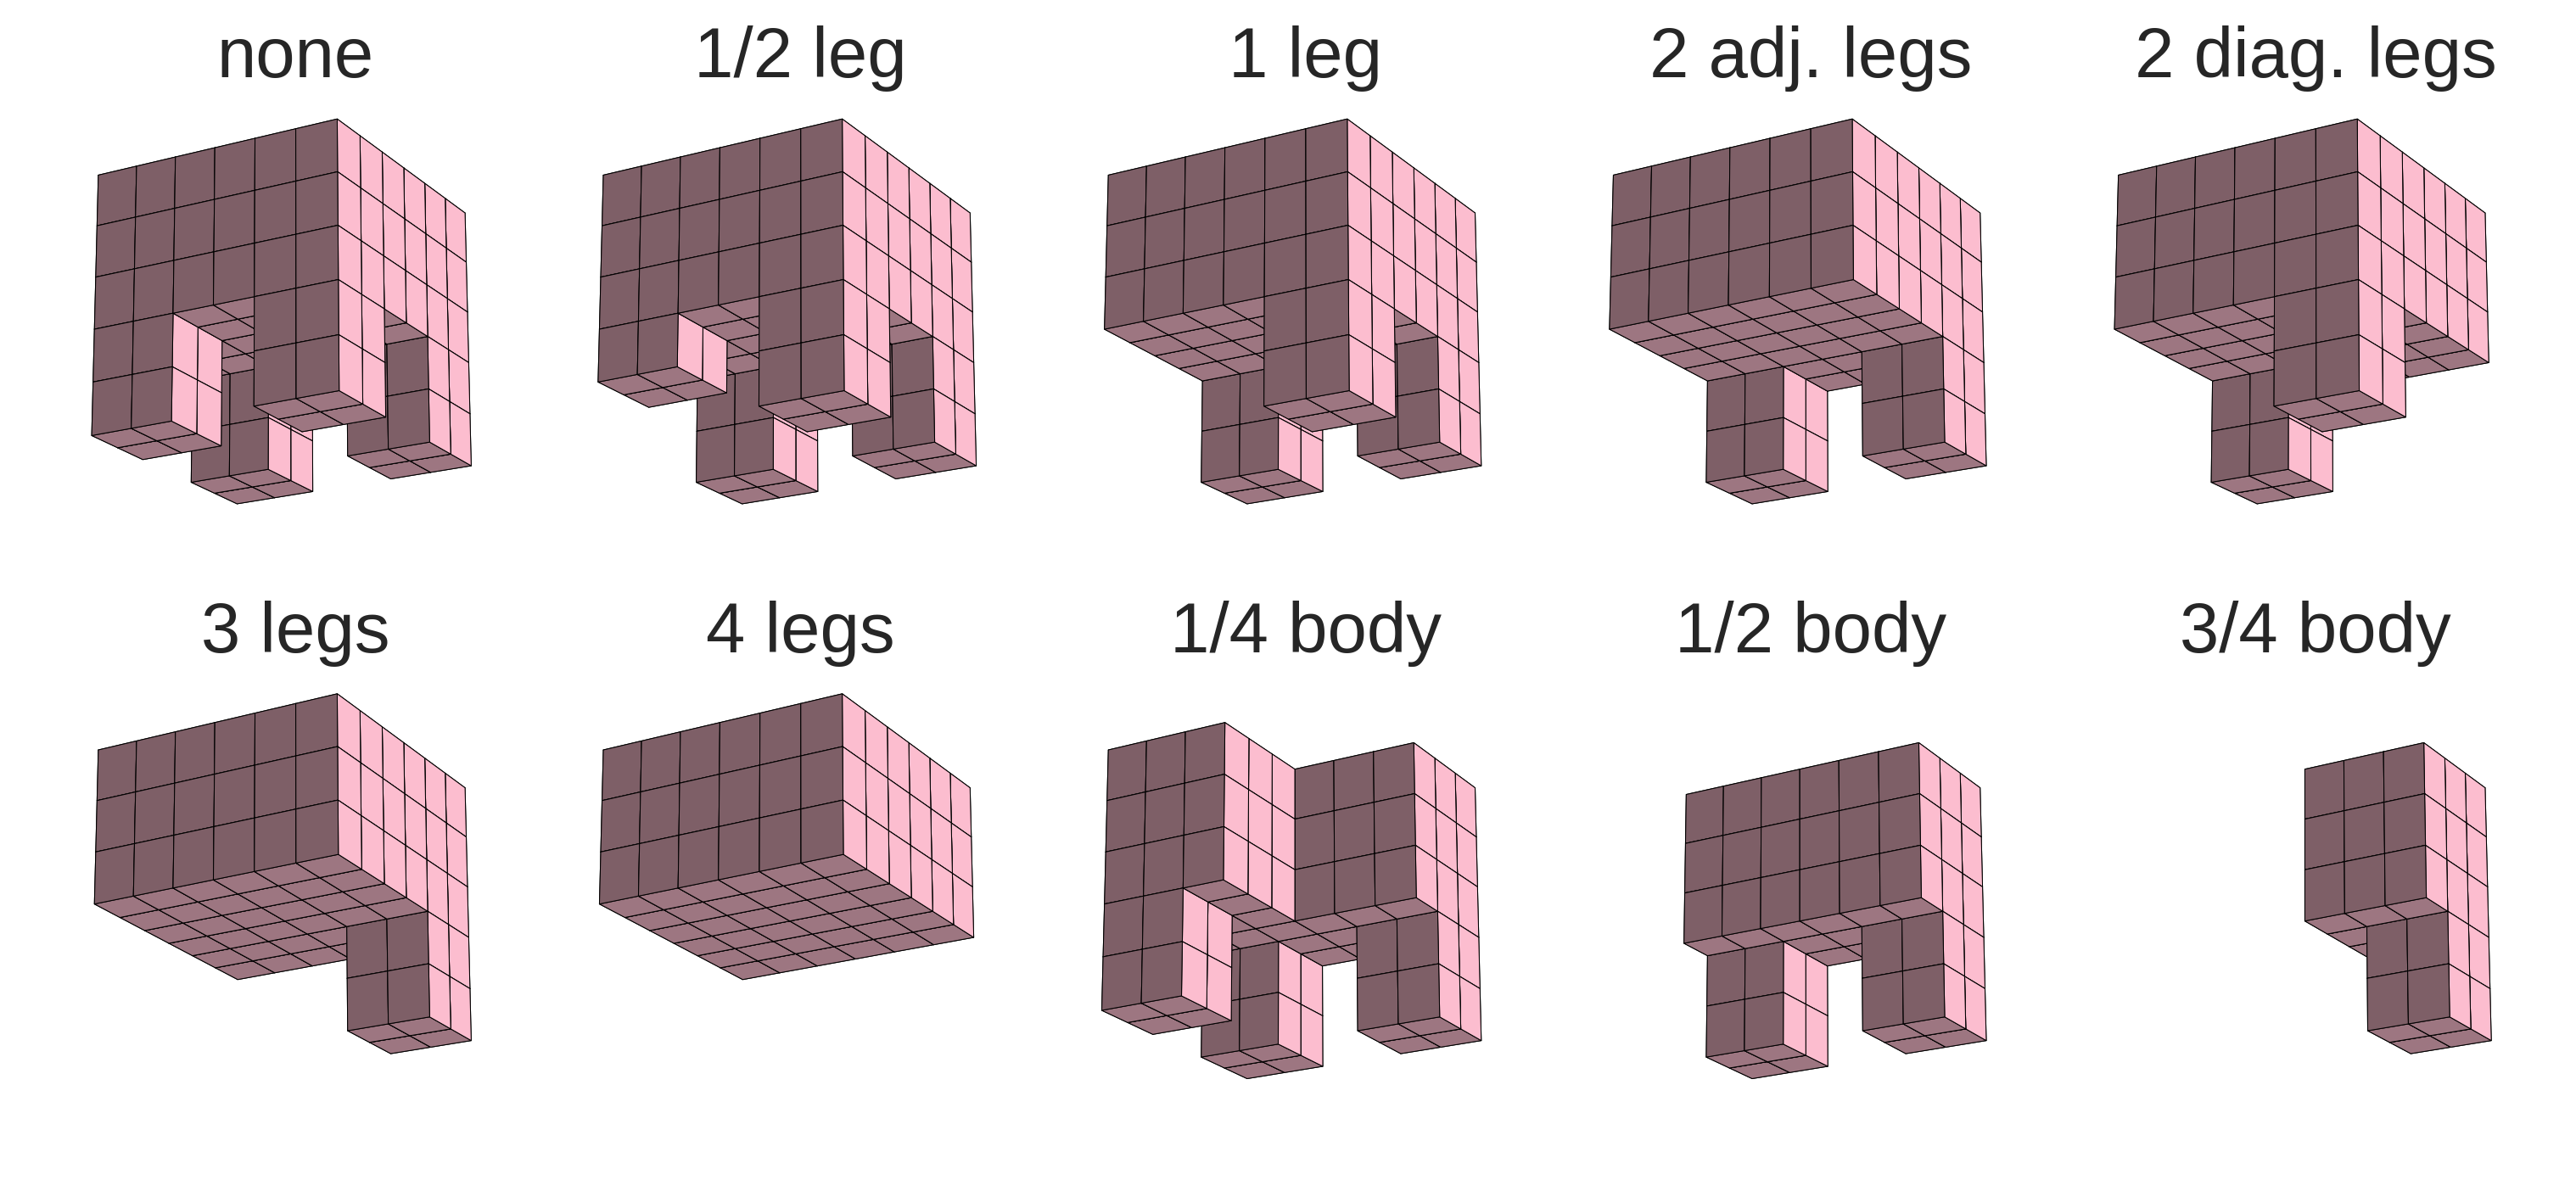
\includegraphics[trim={14pt 0 14pt 0},clip,width=0.9\linewidth]{Chapter05/fig/damage_scenarios.png}\\
% \vspace{-1em}
\caption{\label{fig5:scenarios}The various amputations applied in our experiments. 
The predamage robot (amputation = `none') is shown for reference.}
\vspace{-13pt}
\end{center}
\end{figure}


\subsection*{The recovery options.}


Each damage scenario removes structure and breaks the robot's functionality: the robot loses voxels and its ability to walk.
We here consider two options for function recovery: 
\begin{enumerate}
    \setlength{\itemsep}{3pt}
    \item \textbf{Controller readaptation.}
    A new controller is optimized for locomotion with the damaged structure, as in \cite{bongard2006resilient,cully2015robots}.
    The only parameter subject to (re)optimization is the phase offset, $\phi_i$, of each voxel.
    \item \textbf{Shapeshifting.} The shape of the damaged structure is optimized for locomotion with the existing controller.
    The only parameter subject to optimization is the baseline rest length, $b_i$, of each voxel.
\end{enumerate}


\subsection*{The shape change.}


The body is reshaped 
\textit{prior to} behavior (i.e., before the controller is turned on), analogous to a prenatal developmental stage.
This is done by adjusting the robot's shape, $\mathcal{S}$, as defined in Eq.~\ref{eq5:shape}.
Then, behavior results from oscillations that are symmetrically distributed about this shape 
(Eq.~\ref{eq5:beam_configuration}). 

The same kind of neural network that encodes controllers 
(i.e, a CPPN) 
was also used to encode 
the robot's shape.
However, the 
shape-encoding
networks output a rest beam length, $b_i$, between 0.25 and 2 cm (instead of a phase offset, $\phi_i$, between $-2\pi$ and $2\pi$).
Subject to the constraints outlined above,
optimization searches for shape-encoding networks that result in resting shapes that, when coupled with the original open-loop controller (previously optimized for the undamaged robot), synergize to recover forward movement.


\subsection*{The optimization algorithm.}
\label{sec5:optimization}


Shapes and control policies
are here optimized to displace the (simulated) robot in any direction using Age-Fitness-Pareto Optimization \citep{schmidt2011age}, 
an evolutionary algorithm that uses the concept of Pareto dominance and an objective of `age' (in addition to displacement) intended to promote diversity among candidate designs and prevent premature convergence.

 
A trial is initialized with a population of 50 randomly-generated designs with age zero.
Every generation, the population is first doubled by creating modified copies of each individual in the population (i.e., offspring, in which `age' is set equal to that of the parent), where modification occurs only to the encoding-network that is currently being optimized (either that of $\phi$ or $b$).
The age of each individual is then incremented by one. 
Next, an additional random individual (with age zero) is injected into the population (which now consists of 101 designs). 
Finally, selection reduces the population to its original size (50 designs) according to the two objectives of net displacement (maximized) and age (minimized): Starting with nondominated designs ($N=0$), successive Pareto fronts (containing designs dominated by exactly $N$ alternatives, for $N=1,2,\ldots$) are kept in their entirety until doing so would overfill the population past its original size; then, designs are selected one-by-one with probability proportional to their net displacement. (The 51 unselected designs are deleted.)


This process of random variation and directed selection is repeated for 
$G$ generations, in which
both the architectures and weights of the encoding networks are optimized:
Mutations add, modify or remove a particular vertex or edge.
Where modification of an edge reweights it (within -1 to 1 bounds) by adding a value randomly drawn from a normal distribution with mean zero and standard deviation 0.5.
Vertex modification swaps the node's activation function with a randomly chosen function in the set (adopted from \cite{kriegman2018interoceptive}): sin(), abs(), square(), sqrt(abs()); and the negations of those four. 

